\documentclass{article}
\usepackage[margin=1in]{geometry}
\usepackage{graphicx}
\usepackage{caption}
\usepackage{amsmath}

\title{Startup for Pressurization System}
\author{JC Vaught, William Wenzel, Tanner Harmon, Presston McConnell}
\date{}

\begin{document}
\maketitle

\section*{What you’ll need}
\begin{itemize}
  \item A garden hose
  \item A flashlight
\end{itemize}

\section{Safety Check}
\begin{enumerate}
  \item Walk around the pump house and rainwater tank.
  \item Look closely at every pipe, wire, and fitting.
  \item Make sure you do not see water dripping or pooling, cracked or loose pipes, exposed or dangling wires
  \item If anything looks damaged or wet, stop and refer to the troubleshooting or repair guide before you proceed.
\end{enumerate}

\section{Open the Main Water Valve}
\begin{enumerate}
  \item Go to the big green rainwater tank (capacity: 1,000~gallons).
  \item Find the PVC pipe coming out of the tank with a black handle on top (see Figure~\ref{fig:main_valve}).
  \item Rotate the handle 90° so it lines up with the pipe — this means it’s fully open.
\end{enumerate}

\begin{figure}[h]
  \centering
  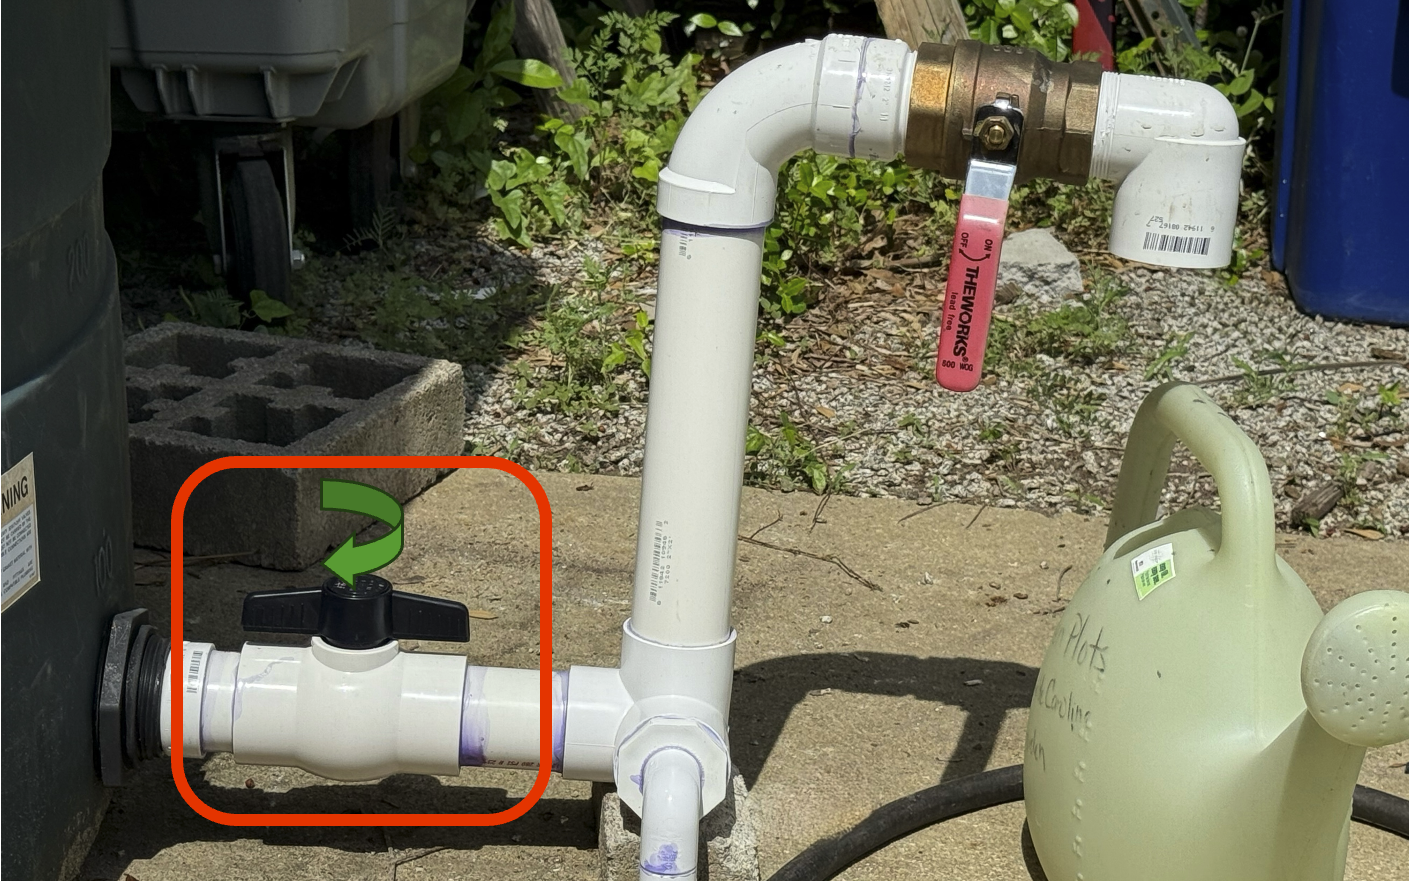
\includegraphics[width=0.65\textwidth]{main_valve.png}
  \caption{Main water-feed valve by the rainwater tank. Turn the black handle 90° until it lines up with the pipe to open.}
  \label{fig:main_valve}
\end{figure}

\section{Power Up the Pump}
\begin{enumerate}
  \item Enter the pump house and turn on the light.
  \item Locate the inverter mounted on the wall (a grey box labeled “OUTPUT 115V/60Hz AC”) (see Figure~\ref{fig:inverter}).
  \item Make sure the pump’s power cord is firmly plugged into the inverter’s outlet — or, if you have a Low Water Detector (LWD) installed, plug it into the LWD first.
    \begin{itemize}
      \item If it’s unplugged, push it in firmly until it clicks.
    \end{itemize}
  \item Flip the red switch on the inverter to the “I” (ON) position.
    \begin{itemize}
      \item A green light next to the switch should glow.
    \end{itemize}
\end{enumerate}

\begin{figure}[h]
  \centering
  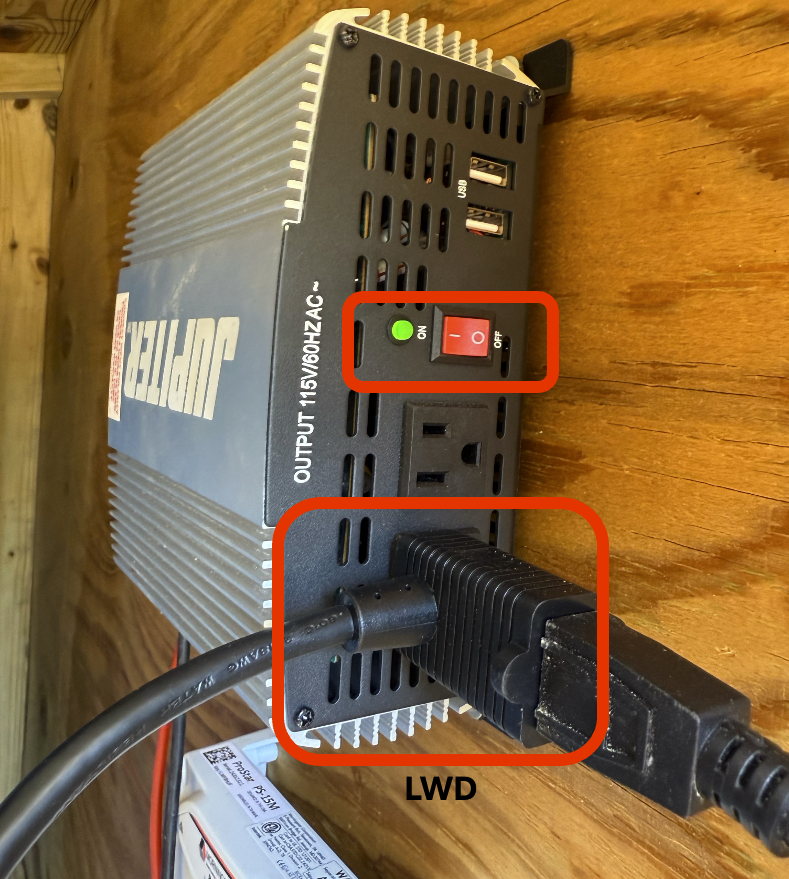
\includegraphics[width=0.6\textwidth]{inverter.png}
  \caption{Inside the pump house: the inverter unit with its red ON/OFF switch and green power indicator. Ensure the pump’s cord (or the Low Water Detector, if installed) is plugged firmly into the inverter outlet before switching it on.}
  \label{fig:inverter}
\end{figure}

\section{Wait for Pump to Build Pressure}
\begin{enumerate}
  \item Once powered, the pump will run and draw water from the tank.
  \item Listen for the pump motor. It will run until the system reaches its target pressure.
  \item When the pressure is high enough, the pump will automatically stop.
\end{enumerate}

\section{Use the Water Spigot}
\begin{enumerate}
  \item Go back outside to the side of the pump house.
  \item Find the brass spigot with the red handle (see Figure~\ref{fig:spigot}).
  \item Attach your garden hose to the spigot’s threaded nozzle.
  \item Turn the red handle 90° so it lines up with the hose — this opens the faucet.
  \item Water will flow through your hose at the set pressure.
\end{enumerate}

\begin{figure}[h]
  \centering
  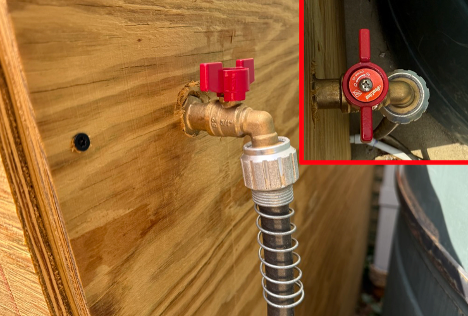
\includegraphics[width=0.9\textwidth]{out_spigot.png}
  \caption{Outdoor brass spigot on the pump house wall. Attach your hose to the threaded outlet and turn the red handle until it’s parallel with the pipe to start the flow.}
  \label{fig:spigot}
\end{figure}

\section*{When You’re Done}
\begin{itemize}
  \item Turn the red handle on the spigot perpendicular to the pipe (off position).
  \item Do not turn off the system unless winterizing or repairing the system.
\end{itemize}

\end{document}
